\documentclass[25pt,a1paper]{tikzposter} %size is 84cmX120cm
\usepackage{graphicx}
\graphicspath{{pictures}}
\usetheme{Wave} %theme of poster design
\usetitlestyle{Wave}
\usepackage{lipsum} %for dummy text
\usepackage{multicol}

\begin{document}
    \title{This is an Amazing Poster}
    \author{Sampath Singamsetty}
    \maketitle

    \begin{columns}
    %COLUMN 1
    \column{.65}%use 65% of the available space for this column
    %Block A
    \block{More Examples of LaTeX}{
    \bigskip
    You can even put stuff in colored boxes.\\
    \coloredbox{\begin{itemize}
      \item point 1
      \item point 2
    \end{itemize}}
    \lipsum[2]
    \bigskip
    \innerblock{Some fun with mathematics}{
        \begin{center}
                \[
                    \int_a^b f(x) dx \approx (b - a)
                    \sum_{i=0}^n w_i f(x_i)
                \]
        \end{center}
        }
    }
    \note[targetoffsetx = 4cm,targetoffsety = -9cm,angle = -25,connection,width = 9cm]{A Weight function}
    %Block B 
    \block{More Text}{\lipsum[2]}

    %COLUMN 2
    \column{.35} %last 1/3 of space
    \block{More Pictures}{
        \begin{center}
            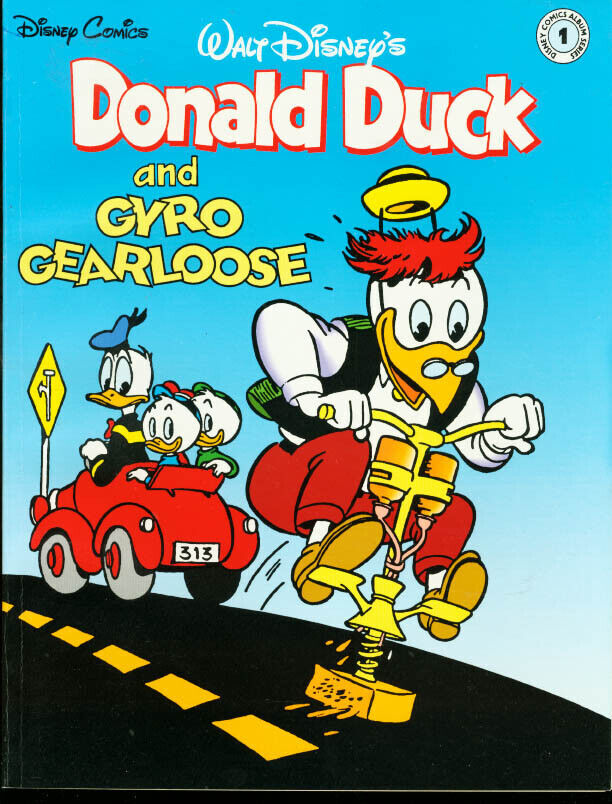
\includegraphics[width=0.9\linewidth]{gyro}
        \end{center}
        \lipsum[4]
    }
    \end{columns}
    \block{The End}{
    \lipsum[11-12]
    }
\end{document}
